There are a number of different kind of language processors, however, we focus on the ones important to our project: Translators. A translator is exactly what it sounds like; it is a program that translates one language into another, this being Chinese into English, or C\# into Java. \\ \indent 
   In particular, we will focus on two types of translators; Compilers and interpreters. We descripe the usage of them, and differences and similarities between them.

\section{Compilers}
A compiler is basically a translator, typically capable of translating a language with a high level of abstraction (high level language), into a language that has a low level of abstraction (low-level language). This could for example translate the language C into runnable machine code. A compiler has the defining property that it has to translate the entire input before the result can be used, however, it will then be run at full machine speed. If the input is very large it may take quit a while to finish translating, other then that there are no disadvantages to the approach.\\ \indent

A basic compiler can be broken down to three simple steps, which are illustrated in \ref{fig:compiler}.

\begin{figure}[H]
\begin{center}
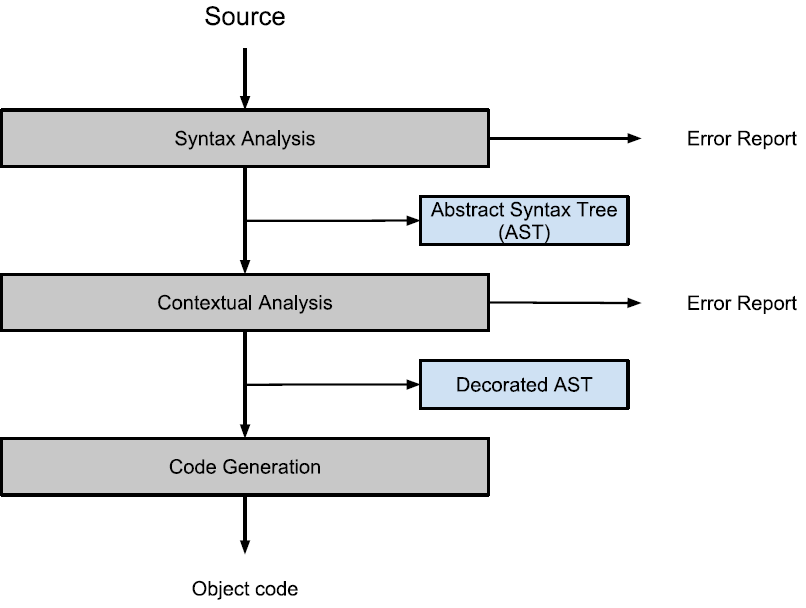
\includegraphics[scale=0.5]{Images/compiler_drawing.png}
\label{fig:compiler}
\caption{Illustration of the general structure of the compiler components.}
\end{center}
\end{figure}


\section{Interpreters}
An interpreter is also a translator, but where the compiler has to translate the entire input before the results can be used, the interpreter runs one instruction at a time from the input, thus enabling it to start utilizing the input right when it receives it. This boosts the time it will initially take to start running the output, but reduces the speed at which it can be run.,\\
\indent Because of this people would normally say that an Interpreter is best used when the program does not have to be run a great many times, or when the program in under development, and a compiler is best used when releasing large scale distributions of program.